\chapter{Perancangan Perangkat Lunak}
\label{chap:perancangan}

	Pada bab ini akan dibahas mengenai detil-detil dari perangkat lunak optimisasi algoritma ant colony
	untuk kasus multi objective flow shop. Struktur kelas dan hal-hal yang mampu dilakukan  melalui perangkat 
	lunak ini juga akan dijabarkan.
	
\section{Perancangan Antarmuka Grafis}
	
	Untuk mempermudah penggunaan, perangkat lunak akan memiliki sebuah interface. Interface ini
	dibuat agar pengguna perangkat lunak dapat dengan mudah menjabarkan kasus flow shop yang ingin dioptimisasi. 
	Interface ini juga dibuat agar proses optimisasi yang dilakukan dapat lebih mudah dipantau. Melalui interface ini, 
	pengguna dapat memberikan data masukan kasus flow shop lewat sebuah file teks. 
	Pengguna juga dapat mengetahui hasil optimisasi yang diberikan pada setiap fase pelatihan.
	
	Berikut tampilan {\it interface} tersebut : 
	\begin{figure}[H]
		\centering
		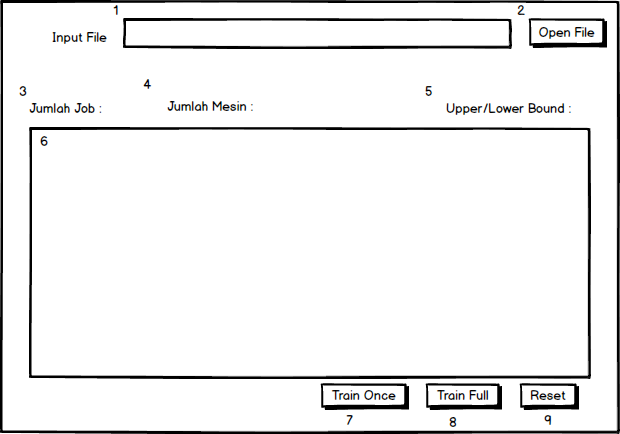
\includegraphics[scale=0.65]{RancanganGrafis}
		\caption[Rancangan {\it interfcae} perangkat lunak]{Rancangan {\it interface} perangkat lunak}
		\label{fig:rancanganinterface}
	\end{figure}
	
	Keterangan dari {\it interface} tersebut sebagai berikut :
	\begin{enumerate}
		\item Memberitahu informasi nama {\it file} teks yang telah dipilih pengguna untuk dioptimisasi.
		\item Memilih {\it file} teks yang berisi satu kasus flow shop. File yang dipilih harus berupa file.txt. 
		Agar {\it file} dapat dikonversi menjadi sebuah kasus flow shop, data di dalam file tersebut juga harus sesuai 
		dengan format penulisan yang sudah ditentukan.
		\item Menampilkan banyaknya pekerjaan yang ada pada kasus flow shop yang dipilih.
		\item Menampilkan banyaknya mesin yang ada pada kasus flow shop yang dipilih.
		\item Menampilkan informasi nilai upper bound dan lower bound dari kasu flow shop yang dipilih.
		\item Menampilkan informasi mengenai solusi optimal yang diberikan pada setiap proses pelatihan.
		Informasi yang diberikan berupa urutan pengerjaan yang dilakukan, nilai makespan yang
		dihasilkan,nilai waiting time mesin, dan pada proses pelatihan ke berapa solusi tersebut didapatkan.
		\item Melakukan proses pelatihan dengan menggunakan algoritma ant colony sebanyak 1 kali pada
		kasus flow shop yang dipilih.
		\item Melakukan proses pelatihan dengan menggunakan algoritma ant colony pada kasus flow shop yang dipilih hingga 
		kondisi berhenti dicapai. Kondisi berhenti yang digunakan adalah diberikannya solusi optimal yang sama pada 10 proses pelatihan terakhir.
		\item Mengulang kembali proses optimisasi dari fase pelatihan pertama.
	\end{enumerate}

\section{Diagram Kelas Lengkap}
	
	Perangkat lunak akan dibuat secara {\it Object Oriented }. Kelas-kelas yang dibuat akan memperhatikan
	kebutuhan dan keterhubungan dari masing-masing objek yang terlibat. Interface yang akan dibuat
	akan langsung memiliki keterhubungan dengan kelas yang mampu melakukan proses optimisasi.
	Keterhubungan tersebut tidak diperantara oleh kelas Controller seperti pada topologi {\it Model }, {\it View },
	dan {\it Controller }.
	\newpage
	Berikut adalah diagram kelas dari perangkat lunak yang dibuat.
	\begin{figure}[H]
		\centering
		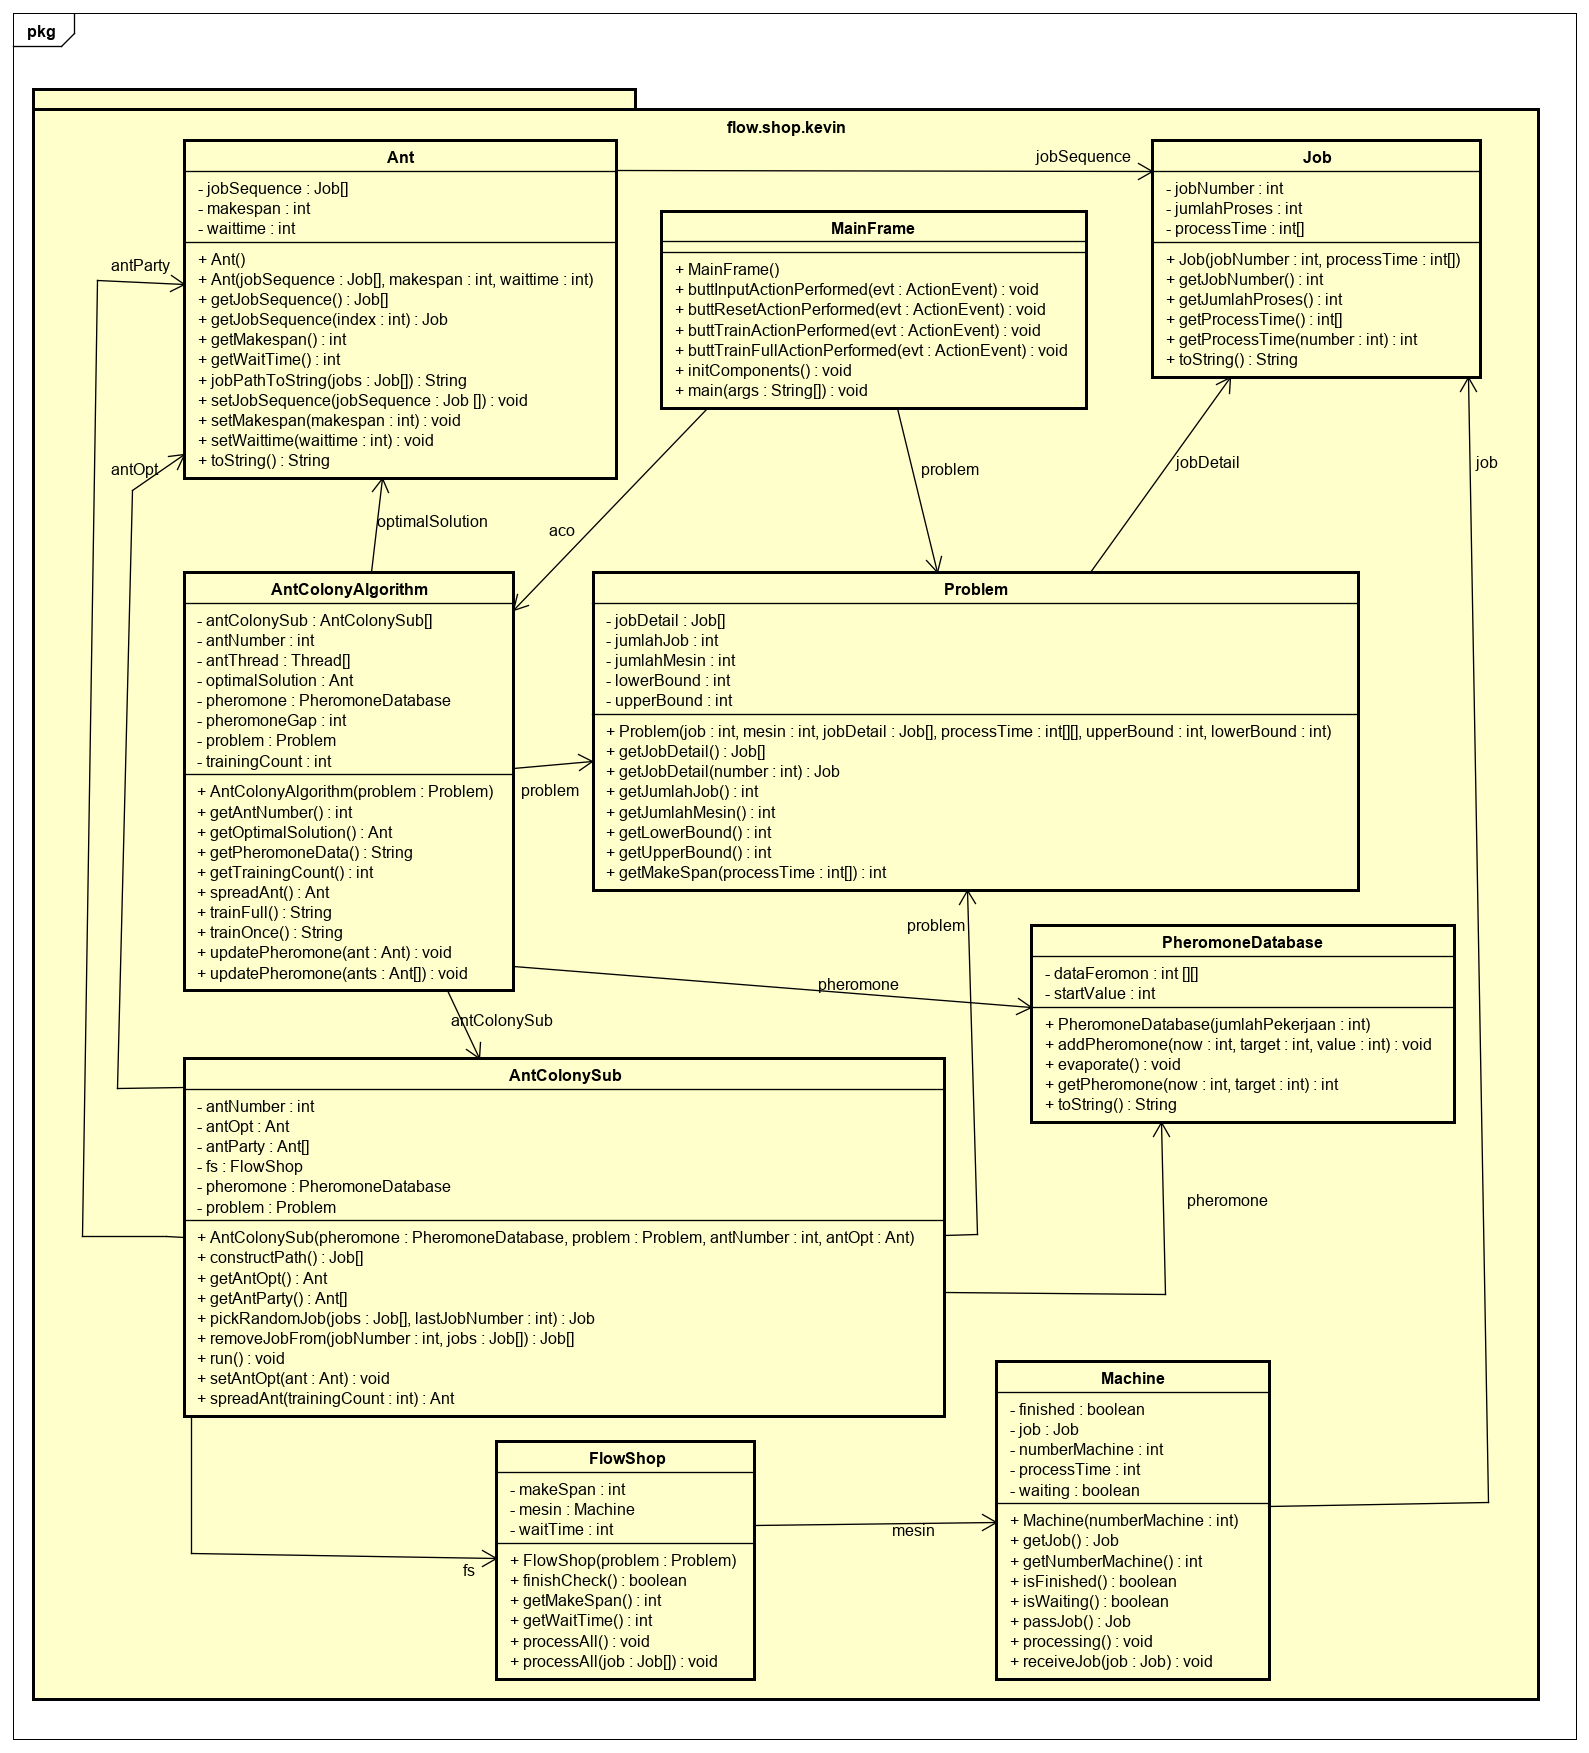
\includegraphics[scale=0.42]{ClassDiagramLengkap}
		\caption[Diagram kelas dari perangkat lunak]{Diagram kelas dari perangkat lunak}
		\label{fig:diagramkelas}
	\end{figure}
	
	Penjelasan dari diagram kelas : 
	\begin{itemize}
		\item \textbf{Kelas MainFrame} \\
		Kelas ini merupakan kelas yang membentuk { \it interface } dan mengaplikasikan fungsi-fungsi aplikasi
		pada komponen-komponen {\it interface }. {\it Interface } yang dibentuk oleh kelas ini berguna
		untuk proses interaksi dengan pengguna selama perangkat lunak dijalankan. Atribut dan
		method yang dimiliki oleh kelas ini adalah :
		
		\begin{itemize}
			\item Atribut 
			\begin{itemize}
				\item problem \\
				Kasus flow shop yang telah dikonversi dari file teks dan ingin dicari hasil
				optimalnya.
				\item aco \\
				Algoritma ant colony yang digunakan untuk pencarian hasil optimal dari kasus flow shop yang disimpan
				pada atribut problem.
			\end{itemize}
			\item Method 
			\begin{itemize}
				\item MainFrame \\
				{\it Constructor } dari kelas ini.
				\item initComponents \\
				Menginisialisasikan komponen-komponen seperti Tombol, {\it Text Box }, dan {\it Text Area}
				pada {\it interface }.
				\item buttInputActionPerformed \\
				Membuat kotak dialog baru untuk memilih file teks berisi kasus flow shop
				yang ingin dicari hasil optimalnya. Method ini akan mengkonversi file teks tersebut
				menjadi kasus flow dan mengkonfigurasi algoritma ant colony yang
				akan digunakan untuk pencarian hasil optimal dari kasus tersebut. Method ini akan
				dijalankan saat pengguna menekan tombol "Browse".
				\item buttTrainActionPerformed \\
				Melakukan proses pelatihan dengan menggunakan algoritma ant colony sebanyak
				1 kali pada kasus flow shop yang dipilih. Hasil dari proses optimisasi akan
				ditampilkan pada pengguna. Method ini akan dijalankan saat pengguna menekan
				tombol "Train Once".
				\item buttResetActionPerformed \\
				Mengulang kembali proses optimisasi dari kondisi awal. Method ini akan dijalankan
				saat pengguna menekan tombol "Reset".
				\item buttTrainFullActionPerformed \\
				Melakukan proses pelatihan dengan menggunakan algoritma ant colony pada kasus flow shop 
				yang dipilih hingga kondisi berhenti dicapai. Kondisi berhenti yang
				digunakan adalah diberikannya solusi optimal yang sama pada 10 proses pelatihan
				terakhir. Hasil dari proses optimisasi hingga kondisi tercapainya kondisi berhenti
				akan ditampilkan pada pengguna. Method ini akan dijalankan saat pengguna menekan
				tombol "Train Full".
				\item main \\
				Method untuk menginisialisasi dan menjalankan perangkat lunak.
			\end{itemize}
			
		\end{itemize}
	
		\item \textbf{Kelas Job} \\
		Kelas ini merepresentasikan sebuah pekerjaan yang akan dikerjakan pada sebuah kasus flow shop. 
		Kelas ini menyimpan informasi-informasi mengenai sebuah pekerjaan pada kasus flow shop. 
		Atribut dan method yang dimiliki oleh kelas ini adalah :
		
		\begin{itemize}
			\item Atribut 
			\begin{itemize}
				\item jobNumber \\
				Menyimpan nomor petunjuk identitas sebuah pekerjaan. Atribut ini merupakan
				nomor pembeda sebuah pekerjaan dari pekerjaan lainnya dalam sebuah kasus flow shop.
				\item processTime \\
				Menyimpan detil waktu pengerjaan proses-proses pada sebuah pekerjaan. Detil-detil
				waktu proses tersebut disimpan dalam bentuk array integer. Indeks array berfungsi
				sebagai penunjuk nomor proses dari pekerjaan tersebut.
				\item jumlahProses \\
				Menyimpan detil mengenai banyaknya proses dalam sebuah pekerjaan. Nilai atribut
				ini diberikan pada saat pembentukkan kelas. Nilai dari atribut ini sesuai dengan
				panjang array integer dari atribut processTime.
			\end{itemize}
			\item Method
			\begin{itemize}
				\item job \\
				Contructor dari kelas ini. Pembuatan kelas ini dilakukan saat mengkonversi file teks
				menjadi suatu kasus flow shop. Adapun parameter-parameter yang diperlukan
				untuk pembentukkan kelas ini adalah : 
				\begin{itemize}
					\item jobNumber : nomor / nama pekerjaan.
					\item processTime : detil waktu proses pekerjaan, dalam bentuk array integer.
				\end{itemize}
				\item toString\\
				Method ini akan mengembalikan detil waktu-waktu proses pada sebuah pekerjaan.
				Detil waktu tersebut akan ditampilkan dalam sebuah String yang akan diberikan
				kepada pengguna perangkat lunak.
				\item getJobNumber\\
				Method ini akan mengembalikan nilai atribut jobNumber yang berisi nomor identitas dari pekerjaan.
				\item getProcessTime\\
				Method ini akan mengembalikan nilai atribut processTime yang berisi detil waktu
				proses dari pekerjaan ini. Atribut ini akan diberikan dalam bentuk array
				integer. Method ini juga mampu menerima parameter sebuah angka integer sebagai
				penunjuk nomor proses. Jika method ini menerima parameter nomor proses tersebut,
				maka method ini akan mengembalikan sebuah integer lama waktu pengerjaan
				proses ke-x dari pekerjaan tersebut, di mana x tersebut merupakan parameter nomor
				pekerjaan yang dimasukkan.
				\item getJumlahProses\\
				Method ini akan mengembalikan nilai atribut jumlahProses yang berisi banyaknya
				proses pada pekerjaan ini.
			\end{itemize}
		\end{itemize}
		
		\item \textbf{Kelas Problem} \\
		Kelas ini merepresentasikan sebuah kasus flow shop. Kelas ini menyimpan informasi - informasi pada suatu kasus flow shop.
		Atribut dan method yang dimiliki oleh kelas ini adalah :
		
		\begin{itemize}
			\item Artribut
			\begin{itemize}
				\item jumlahJob \\
				Menyimpan informasi mengenai banyaknya pekerjaan pada sebuah kasus flow shop.
				\item jumlahMesin \\
				Menyimpan informasi mengenai banyaknya perangkat mesin yang mampu mengerjakan
				masing-masing proses.
				\item jobDetail \\
				Menyimpan informasi mengenai setiap pekerjaan yang terdapat pada kasus flow shop. 
				Informasi disimpan dalam bentuk array kelas Job. Indeks array berfungsi
				sebagai penunjuk nomor pekerjaan.
				\item upperBound \\
				Menyimpan informasi nilai upper bound dari kasus flow shop.
				\item lowerBound \\
				Menyimpan informasi nilai lower bound dari kasus flow shop.
			\end{itemize}
			\item Method
			\begin{itemize}
				\item Problem\\
				Constructor dari kelas ini. Pembuatan kelas ini merupakan hasil konversi file teks menjadi 
				sebuah kasus flow shop. Parameter-parameter yang dibutuhkan untuk pembentukkan kelas ini adalah :
				\begin{itemize}
					\item job : banyaknya pekerjaan.
					\item mesin : banyaknya perangkat mesin.
					\item jobDetail : informasi pekerjaan-pekerjaan yang ada, dalam bentuk array kelas Job.
					\item processTime : pembentukan waktu proses dari setiap job, berdasarkan mesin dan job. Akan digunakan
					pada kelas MainFrame.
					\item upperBound : nilai upper bound.
					\item lowerBound : nilai lower bound.
				\end{itemize}
				\item getJumlahJob \\
				Mengembalikan nilai atribut jumlahJob yang berisi informasi mengenai banyaknya
				pekerjaan pada kasus flow shop.
				\item getJobDetail \\
				Mengembalikan detil informasi mengenai pekerjaan yang ada pada kasus flow shop. 
				Method ini akan mengembalikan informasi detil pekerjaan dalam bentuk array
				kelas Job. Method ini juga mampu menerima sebuah parameter number, di mana
				number merupakan penunjuk nomor / nama pekerjaan. Jika method ini menerima
				parameter tersebut, maka method ini akan mengembalikan informasi pekerjaan dengan
				nomor / nama pekerjaan tersebut. Informasi tersebut diberikan dalam bentuk sebuah objek 
				dari kelas Job.
				\item getJumlahMesin \\
				Mengembalikan detil informasi mengenai banyaknya perangkat mesin yang ada pada
				kasus flow shop.
				\item getUpperBound \\
				Mengembalikan nilai upper bound pada kasus flow shop yang disimpan pada
				atribut upperBound
				\item getLowerBound \\
				Mengembalikan nilai lower bound pada kasus flow shop yang disimpan pada
				atribut lower Bound.
			\end{itemize}
		\end{itemize}
	
		\item \textbf{Kelas Machine} \\
		Kelas ini merepresentasikan sebuah mesin pada sistem penjadwalan flow shop. Kelas ini
		menjabarkan kondisi mesin yang sedang mengerjakan / menunggu sebuah pekerjaan. Atribut
		dan method yang dimiliki oleh kelas ini adalah :
		
		\begin{itemize}
			\item Atribut
			\begin{itemize}
				\item job \\
				Menyimpan informasi mengenai pekerjaan yang sedang dikerjakan / disimpan pada
				mesin ini. Informasi disimpan dalam bentuk sebuah objek dari kelas Job.
				\item numberMachine \\
				Menyimpan informasi mengenai banyaknya mesin.
				\item processTime \\
				Menyimpan informasi mengenai lama waktu proses yang telah dilalui dalam pengerjaan
				proses dari sebuah pekerjaan. Jika pekerjaan telah selesai dikerjakan / tidak
				ada pekerjaan pada mesin, maka atribut ini akan bernilai 0.
				\item finished
				Menyimoan informasi mengenai status mesin. 
				Atribut ini mengindentifikasikan sebuah mesin telah menyelesaikan pekerjaannya.
				\item waiting \\
				Menyimpan informasi mengenai status mesin. Atribut ini mengindentifikasikan sebuah
				mesin sedang kosong dan menunggu pekerjaan baru untuk dikerjakan.
			\end{itemize}
			\item Method
			\begin{itemize}
				\item Machine \\
				Constructor dari kelas ini. Pembuatan kelas ini dilakukan pada saat konfigurasi
				mesin-mesin pada sistem flow shop agar sesuai dengan kasus flow shop yang ingin dikerjakan / dioptimisasi.
				Parameter yang diperlukan dalam pembentukkan kelas ini adalah :
				\begin{itemize}
					\item numberMachine : banyaknya mesin yang ada pada kasus flow shop
				\end{itemize}
				Pada saat pembentukkan objek dari kelas ini, mesin akan dianggap sebagai sebuah
				mesin baru tanpa ada pekerjaan apapun yang dikerjakan di dalamnya. Oleh karena
				itu, nilai dari atribut job akan bernilai null. Nilai dari atribut processTime akan
				bernilai 0. Nilai dari atribut \textit{waiting} dan \textit{finished} akan bernilai \textit{true}.
				\item processing \\
				Menambah 1 nilai pada atribut processTime. Jika nilai dari atribut processTime
				telah sama dengan waktu pengerjaan dari proses pekerjaan yang ditugaskan pada
				mesin, maka method ini akan mengubah status mesin menjadi sudah selesai mengerjakan
				tugasnya. Status mesin yang sudah selesai mengerjakan tugasnya ditandai
				dengan atribut \textit{finished} yang bernilai \textit{true}. Jika mesin telah menyelesaikan tugasnya,
				maka nilai dari atribut processTime juga akan diatur ulang menjadi bernilai 0.
				Method ini hanya akan berjalan pada mesin dengan nilai atribut finished \textit{false}.
				\item passJob \\
				Mengoper pekerjaan yang telah diselesaikan oleh mesin. Method ini akan mengembalikan
				pekerjaan yang telah diselesaikan oleh mesin dalam bentuk sebuah objek dari
				kelas Job. Pada saat yang sama, method ini juga akan mengubah status mesin menjadi
				kosong / menunggu pekerjaan baru. Mesin yang sedang menunggu pekerjaan
				baru ditandai dengan berubahnya nilai dari atribut \textit{waiting} menjadi \textit{true}. Method ini
				juga akan mengatur ulang nilai dari atribut job menjadi null. Method ini hanya bisa
				dijalankan pada mesin dengan nilai atribut \textit{finished true} dan nilai atribut \textit{waiting false}. 
				Nilai atribut tersebut dapat diartikan sebagai mesin yang sudah menyelesaikan pekerjaannya tetapi masih menyimpan pekerjaannya.
				\item receiveJob \\
				Menerima pekerjaan baru untuk dikerjakan mesin. Method ini menerima sebuah
				parameter berupa objek dari kelas Job, di mana parameter tersebut merupakan pekerjaan
				baru yang harus dikerjakan oleh mesin. Parameter tersebut akan disimpan
				sebagai atribut job dari mesin. Method ini akan mengubah status mesin menjadi
				sedang mengerjakan sebuah pekerjaan. Mesin yang sedang mengerjakan sebuah pekerjaan
				ditandai dengan atribut \textit{finished} dan \textit{waiting} yang bernilai false. Method ini
				hanya dapat dijalankan pada mesin yang sedang menunggu pekerjaan baru(atribut waiting bernilai \textit{true}).
				\item isWaiting \\
				Mengembalikan informasi mengenai apakah mesin sedang kosong atau tidak. Informasi
				didapat dari atribut waiting. Jika mesin sedang kosong dan sedang menunggu
				diberikannya pekerjaan baru, maka method ini akan mengembalikan nilai boolean
				true. Jika mesin sedang mengerjakan / menyimpan sebuah pekerjaan, maka method
				akan mengembalikan nilai boolean false.
				\item isFinished \\
				Mengembalikan informasi mengenai apakah mesin sudah / belum menyelesaikan pekerjaannya.
				Informasi tersebut didapatkan dari atribut finished. Jika mesin telah menyelesaikan proses dari 
				pekerjaan di dalamnya, maka method ini akan mengembalikan nilai boolean true. Jika mesin belum
				menyelesaikan pekerjaannya, maka method akan mengembalikan nilai boolean false.
				\item getJob \\
				Mengembalikan informasi mengenai pekerjaan yang sedang dikerjakan / disimpan
				oleh mesin. Informasi diberikan dalam bentuk sebuah objek dari kelas Job. Jika
				mesin sedang tidak mengerjakan / menyimpan sebuah pekerjaan, maka method ini
				akan mengembalikan nilai null.
				\item getNumberMachine \\
				Mengembalikan informasi mengenai banyaknya mesin pada kasus flow shop.
			\end{itemize}
		\end{itemize}
		
		\item \textbf{Kelas Flow Shop} \\
		Kelas ini merepresentasikan sebuah sistem penjadwalan flow shop. Kelas ini bertugas
		mengatur kapan sebuah mesin harus menerima dan mengoper sebuah pekerjaan. Kelas ini
		juga bertugas untuk menghitung lama waktu yang dibutuhkan untuk pengerjaan sekumpulan
		pekerjaan dengan urutan tertentu. Atribut dan method yang dimiliki oleh kelas ini adalah :
		
		\begin{itemize}
			\item Atribut
			\begin{itemize}
				\item mesin \\
				Informasi mengenai rangkaian mesin yang ada pada sistem flow shop. Informasi
				disimpan dalam bentuk array 1 dimensi dari kelas Mesin. Indeks dari array menunjukkan 
				nomor mesin. Sebagai contoh indeks array [2] dari atribut
				ini menunjuk pada mesin kedua .
				\item makespan \\
				Menyimpan informasi mengenai nilai makespan yang dihasilkan dari urutan pengerjaan.
				\item waittime \\
				Menyimpan informasi mengenai nilai waktu tunggu mesin dalam memproses suatu kasus flow shop.
			\end{itemize}
			\item Method 
			\begin{itemize}
				\item FlowShop \\
				Constructor dari kelas ini. Pembentukkan kelas ini dilakukan pada saat konfigurasi
				sistem flow shop agar sesuai dengan kasus flow shop yang ingin dikerjakan
				/ dioptimisasi. Parameter yang dibutuhkan untuk pembentukkan kelas ini
				adalah :
				\begin{itemize}
					\item problem : kasus flow shop yang ingin dikerjakan / dioptimisasi.
				\end{itemize}
				Pada saat pembentukkan sebuah sistem flow shop, konfigurasi rangkaian mesin
				pada sistem flow shop akan dilakukan. Banyaknya perangkat mesin untuk
				setiap proses akan diatur berdasarkan nilai-nilai yang ada pada parameter kasus
				flow shop. Nomor proses yang harus dikerjakan masing-masing mesin juga
				akan diatur secara otomatis.
				\item processAll \\
				Method ini akan menghitung nilai makespan dan nilai waittime yang dihasilkan oleh parameter ar-
				ray kelas Job yang dimasukkan. Parameter tersebut dianggap sebagai sekumpulan
				pekerjaan yang akan dimasukkan / dikerjakan oleh sistem flow shop ini.
				Pekerjaan-pekerjaan tersebut akan dikerjakan secara terurut berdasarkan indeks ar-
				ray kelas Job tersebut. Method ini akan menghitung nilai makespan dan nilai waittime yang dihasilkan
				dari suatu solusi / urutan pengerjaan berdasarkan berapa kali method processAll dijalankan.
				
				Method ini akan mengatur kapan proses pengoperan dan penerimaan pekerjaan antar
				mesin terjadi. Method ini juga akan mengatur mesin mana yang berhak melakukan
				pengoperan / menerima sebuah pekerjaan. Proses pengoperan dimulai dengan pengecekan
				mesin-mesin yang mengerjakan proses terakhir dari suatu pekerjaan. Jika
				mesin-mesin tersebut telah menyelesaikan pekerjaannya, maka mesin tersebut akan
				langsung mengoper pekerjaannya tanpa harus ada mesin lain yang menerima pekerjaan
				yang dioper. Pekerjaan yang telah dioper oleh mesin terakhir ini dianggap telah
				selesai dikerjakan. Jika mesin - mesin belum selesai mengerjakan pekerjaannya maka atribut 
				waittime akan bertambah terus . 
				
				Jika terdapat mesin untuk proses selanjutnya yang sedang menunggu pekerjaan baru,
				maka pekerjaan dapat langsung dioper pada mesin tersebut. Jika tidak ada
				mesin untuk proses selanjutnya yang sedang menunggu, maka proses pengoperan
				belum akan dilakukan. Prioritas mengenai mesin yang berhak melakukan pengoperan
				terlebih dahulu ditentukan berdasarkan nomor / nama dari pekerjaan yang akan
				dioper oleh mesin. Jika suatu pekerjaan dikerjakan terlebih dahulu, maka pekerjaan
				tersebut akan memiliki prioritas lebih besar untuk dioper terlebih dahulu.
				
			    Method untuk menghitung nilai makespan dan waittime ini akan terus 
				berjalan selama	masih ada objek dari parameter array kelas Job yang belum dimasukkan ke dalam
				sistem flow shop. Method ini juga akan terus berjalan selama method finishCheck
				mengembalikan nilai true.
				\item finishCheck\\
				Method ini berguna sebagai penanda berhentinya method processAll. Method
				ini akan memeriksa kondisi setiap mesin pada sistem flow shop. Jika setiap
				mesin sedang dalam kondisi menunggu pekerjaan baru (atribut waiting dari kelas
				Mesin bernilai true), maka seluruh pekerjaan yang diberikan dari method processAll
				dapat dianggap telah selesai dikerjakan. Jika seluruh pekerjaan telah selesai
				dikerjakan, maka method ini akan mengembalikan nilai true. Sebaliknya jika terdapat
				salah satu mesin yang tidak dalam kondisi menunggu pekerjaan baru, maka
				method ini akan mengembalikan nilai false.
				\item getMakeSpan \\ 
				Mengembalikan informasi nilai makespan yang dihasilkan oleh urutan pengerjaan /
				solusi.
				\item getWaitTime \\
				Mengembalikan informasi nilai waiitime yang dihasilkan oleh urutan pengerjaan /
				solusi.
			\end{itemize}
		\end{itemize}
		
		\item \textbf{Kelas Ant}\\
		Kelas ini merepresentasikan seekor semut pada algoritma ant colony. Kelas ini akan menyimpan
		sebuah solusi dari hasil proses pembentukan solusi milik algoritma ant colony. Nilai-nilai
		yang disimpan dari seekor semut akan disesuaikan dengan permasalahan yang ingin diselesaikan.
		Dalam kasus ini, nilai yang akan disimpan oleh semut sebagai solusi akan disesuaikan
		dengan permasalahan flow shop. Atribut dan method dari kelas ini adalah :
		
		\begin{itemize}
			\item Atribut
			\begin{itemize}
				\item jobSequence \\
				Menyimpan informasi mengenai salah satu solusi / urutan pengerjaan dari kasus 
				flow shop. Informasi tersebut disimpan dalam bentuk array kelas Job. Indeks
				array menunjukkan nomor urutan pengerjaan.
				\item makespan \\
				Menyimpan informasi mengenai nilai makespan yang dihasilkan dari urutan pengerjaan
				/ solusi yang disimpan pada atribut jobSequence.
				\item waittime \\
				Menyimpan informasi mengenai nilai waktu tunggu mesin dalam memproses suatu kasus flow shop.
			\end{itemize}
			\item Method
			\begin{itemize}
				\item Ant \\
				Constructor dari kelas ini. Pembentukkan kelas ini dilakukan setiap dijalankannya
				fase pelatihan dari algoritma ant colony. Objek dari kelas ini mampu dibentuk langsung
				dengan parameter urutan pengerjaan dan nilai makespan yang ingin disimpan.
				Objek dari kelas ini juga mampu dibentuk tanpa dengan memberikan parameter 
				apapun. Jika objek dibentuk tanpa dengan memasukkan parameter, maka atribut
				jobSequence akan bernilai null dan atribut makespan akan bernilai -1.
				\item toString \\
				Mengembalikan informasi mengenai solusi yang disimpan oleh semut ini secara lengkap.
				Informasi akan diberikan dalam bentuk 3 baris string. Baris pertama menunjukkan
				nilai makespan yang dimiliki, baris kedua merupakan nilai dari waittime dan baris ketiga 
				menunjukkan solusi / urutan pengerjaan yang menghasilkan nilai makespan tersebut.
				\item jobPathToString \\
				Mengkonversi array kelas Job menjadi sebuah string urutan pengerjaan. Pengerjaan
				sebuah pekerjaan ditandai oleh atribut jobNumber dari kelas Job. Perlu diketahui
				pula bahwa perangkat lunak ini membentuk atribut jobNumber pada kelas Job secara
				otomatis dimulai dari nilai 0. Untuk mempermudah penggunaan perangkat lunak,
				method ini akan mengkonversi nilai jobNumber dalam string yang akan diberikan.
				Untuk setiap jobNumber pada string tersebut akan ditambahkan 1. Hal ini dilakukan
				agar pengerjaan pekerjaan pertama didefinisikan dengan jobNumber 1 bukan dengan
				jobNumber 0.
				\item getMakespan \\
				Mengembalikan informasi nilai makespan yang dihasilkan oleh urutan pengerjaan /
				solusi pada atribut jobSequence.
				\item getJobSequence \\
				Mengembalikan informasi urutan pengerjaan yang disimpan oleh semut. Informasi
				diberikan dalam bentuk array kelas Job, dengan indeks array sebagai nomor urutan
				pengerjaannya. Method ini juga mampu menerima sebuah parameter index. Jika
				method dijalankan dengan memberikan parameter tersebut, maka method akan
				mengembalikan informasi mengenai pekerjaan yang dikerjakan di urutan ke index.
				Informasi tersebut diberikan dalam bentuk seuah objek dari kelas Job.
				\item getWaittime \\
				Mengembalikan informasi nilai waiitime yang dihasilkan oleh urutan pengerjaan /
				solusi pada atribut jobSequence.
				\item setJobSequence \\
				Mengubah nilai dari atribut jobSequence sesuai dengan parameter array kelas Job
				yang dimasukkan.
				\item setMakespan \\
				Mengubah nilai dari atribut makespan sesuai dengan nilai parameter yang dimasukkan.
				\item setWaittime \\
				Mengubah nilai dari atribut waittime sesuai dengan nilai parameter yang dimasukkan.
			\end{itemize}
		\end{itemize}
		
		\item \textbf{Kelas PheromoneDatabase} \\
		Kelas ini merepresentasikan tempat penyimpanan nilai feromon untuk panduan proses pembentukan
		solusi secara acak milik algoritma ant colony. Cara penyimpanan nilai feromon
		disesuaikan dengan permasalahan yang ingin diselesaikan. Dalam kasus ini, nilai feromon
		yang disimpan akan disesuaikan dengan permasalahan flow shop dan tata cara yang
		digunakan dalam proses pembentukan solusi secara acak milik algoritma ant colony. Atribut
		dan method yang dimiliki oleh kelas ini adalah :
		
		\begin{itemize}
			\item Atribut
			\begin{itemize}
				\item dataFeromon \\
				Menyimpan informasi mengenai nilai-nilai feromon yang disimpan. Informasi tersebut
				disesuaikan dengan tata cara pembentukkan solusi acak dari algoritma ant
				colony. Informasi disimpan dalam bentuk array 2 dimensi. Indeks pertama dari
				array menunjukkan nomor pekerjaan sebelumnya dan indeks kedua menunjukkan
				nomor pekerjaan selanjuntya.
				\item startValue \\
				Menyimpan informasi mengenai nilai awal yang diberikan pada masing-masing indeks
				atribut dataFeromon. Nilai awal tersebut hanya akan diberikan pada saat
				pembentukkan objek dari kelas ini.
			\end{itemize}
			\item Method
			\begin{itemize}
				\item PheromoneDatabase \\
				Constructor dari kelas ini. Pembentukkan kelas ini dilakukan saat pembentukkan
				kelas AntColonyAlgorithm untuk disesuaikan dengan kasus flow shop yang
				ingin dicari hasil optimalnya. Parameter yang diperlukan untuk pembentukkan kelas
				ini adalah :
				\begin{itemize}
					\item jumlahPekerjaan : banyaknya pekerjaan pada kasus flow shop yang ingin
					dioptimisasi.
				\end{itemize}
				Atribut dataFeromon dari kelas ini akan dibentuk berdasarkan nilai parameter jumlahPekerjaan
				yang dimasukkan. Array yang disimpan pada atribut dataFeromon
				akan berukuran n x n, di mana n merupakan nilai parameter jumlahPekerjaan yang
				dimasukkan. Masing-masing indeks dari atribut dataFeromon akan diberikan nilai
				awal sesuai dengan nilai dari atribut startValue.
				\item getPheromone \\
				Mengembalikan nilai pada suatu indeks dari atribut dataFeromon. Method ini menerima
				2 parameter: \textit{now} dan \textit{target}. Method ini akan mengembalikan nilai dari
				indeks array [now][target] dari atribut dataFeromon.
				\item addPheromone \\
				Menambahkan nilai pada suatu indeks dari atribut dataFeromon. Method ini menerima
				3 parameter: \textit{now}, \textit{target}, dan \textit{value}. Method ini akan menambahkan nilai
				pada indeks array [now][target] dari atribut dataFeromon sejumlah nilai value.
				\item evaporate \\
				Melakukan proses evaporasi feromon pada nilai-nilai feromon yang disimpan. Method
				ini akan mengurangi 30% nilai dari masing-masing indeks pada atribut dataFeromon.
				Nilai hasil evaporasi tidak akan lebih rendah dari 1.
				\item toString \\
				Mengembalikan informasi mengenai nilai-nilai feromon yang disimpan pada atribut
				dataFeromon dalam bentuk string matirks 2 dimensi.
			\end{itemize}
		\end{itemize}
		
		\item \textbf{Kelas AntColonyAlgorithm} \\
		Kelas ini akan melakukan optimisasi dengan menggunakan algoritma ant colony. Kelas ini
		akan mencari urutan pengerjaan yang menghasilkan makespan yang optimal dalam suatu
		kasus flow shop. Dalam mencari hasil optimal tersebut, kelas ini akan dibantu oleh
		kelas PheromoneDatabase. Atribut dan method yang dimiliki oleh kelas ini adalah :
		\begin{itemize}
			\item Atribut
			\begin{itemize}
				\item problem \\
				Menyimpan kasus flow shop yang ingin dicari solusi optimalnya.
				\item pheromone \\
				Menyimpan kelas pheromoneDatabase yang akan membantu dalam pembentukkan
				solusi acak algoritma ant colony.
				\item optimalSolution \\
				Menyimpan solusi optimal dalam bentuk objek dari kelas Ant. Solusi optimal yang
				disimpan merupakan solusi terbaik dari fase-fase pelatihan yang telah dilakukan.
				\item trainingCount \\
				Menyimpan informasi mengenai banyaknya fase pelatihan yang telah dijalankan.
				\item pheromoneGap \\
				Menyimpan informasi mengenai sebuah nilai makespan yang dianggap sebagai nilai
				tengah dari nilai-nilai makespan lainnya yang mungkin dihasilkan. Nilai ini berguna
				dalam menentukan jumlah feromon yang akan ditambahkan dari sebuah solusi acak
				yang telah dibentuk.
				\item antColonySub \\
				Menyimpan informasi mengenai kelompok-kelompok semut yang ada dalam sistem
				algoritma ant colony ini. Masing-masing kelompok akan dijalankan secara bersamaan
				pada saat proses pencarian solusi-solusi lokal dari algoritma ant colony.
				\item antNumber \\
				Menyimpan informasi mengenai banyaknya semut pada setiap kelompok semut.
				\item antThread \\
				Menyimpan informasi thread yang dapat dijadikan penanda selesainya proses pencarian
				solusi / pelatihan dari salah satu kelompok semut.
			\end{itemize}
			\item Method
			\begin{itemize}
				\item AntColonyAlgorithm \\
				Constructor dari kelas ini. Pembentukkan kelas ini dilakukan setelah selesai mengkonversi 
				file teks menjadi suatu kasus flow shop. Parameter untuk pembentukkan
				kelas ini adalah :
				\begin{itemize}
					\item problem : kasus flow shop yang ingin dicari hasil optimalnya.
				\end{itemize}
				Pembentukkan kelas ini akan mengkonfigurasi atribut pheromone dan fs agar sesuai
				dengan kasus flow shop yang ingin dicari hasil optimalnya. Nilai dari atribut
				antNumber akan dibentuk berdasarkan atribut jumlahPekerjaan pada parameter
				kelas Problem yang dimasukkan. Nilai dari atribut pheromoneGap akan disamakan
				dengan nilai makespan yang dihasilkan dari salah satu solusi kasus flow shop.
				Solusi / urutan pengerjaan yang akan dipakai nilai makespan-nya adalah solusi yang
				urutan pengerjaannya terurut berdasarkan nilai atribut jobNumber.
				\item trainOnce \\
				Method ini akan menjalankan proses pelatihan pada algoritma ant colony sebanyak
				satu kali. Method ini akan menjalankan method spreadAnt dengan atribut antNumber
				sebagai parameter. Method ini akan mengembalikan hasil dari proses optimisasi
				tersebut dalam bentuk 3 baris string. Baris pertama menginformasikan banyaknya
				fase pelatihan yang telah dilakukan, baris kedua menunjukkan nilai makespan
				optimal yang diketahui hingga proses pelatihan ini beserta nilai waittime, dan baris 
				ketiga menunjukkan urutan pengerjaan yang menghasilkan nilai makespan tersebut.
				\item trainFull \\
				Method ini akan menjalankan proses pelatihan pada algoritma ant colony hingga
				suatu kondisi berhenti tercapai. Method ini akan menjalankan method spreadAnt
				hingga suatu kondisi berhenti tercapai. Method spreadAnt dijalankan dengan atribut
				antNumber sebagai parameter. Kondisi berhenti yang digunakan adalah diberikannya
				hasil optimisasi yang sama pada 10 fase pelatihan terakhir. Method ini akan
				mengembalikan hasil dari proses optimisasi tersebut dalam bentuk sebuah string.
				String tersebut akan berisi informasi mengenai hasil optimisasi yang diberikan pada
				setiap fase pelatihan hingga kondisi berhenti tersebut tercapai. Masing-masing hasil
				optimisasi pada tiap fase pelatihan dijabarkan dalam 3 baris string. Baris pertama
				menginformasikan nomor fase pelatihan, baris kedua menunjukkan nilai makespan
				optimal yang diketahui hingga proses pelatihan tersebut beserta nilai waittime, dan 
				baris ketiga menunjukkan urutan pengerjaan yang menghasilkan nilai makespan tersebut.
				\item spreadAnt \\
				Method ini akan melakukan fase pelatihan pada algoritma ant colony. Method ini
				akan menginstruksikan masing-masing objek kelas AntColonySub pada atribut untuk
				mulai mencari solusi-solusi lokal. Secara terurut hal-hal yang dilakukan oleh method
				ini adalah :
				\begin{itemize}
					\item Menginstruksikan setiap kelompok semut (atribut antColonySub) untuk memulai
					mencari solusi-solusi dari permasalahan pada atribut problem.
					\item Masing-masing kelompok semut akan :\\
					- Membentuk solusi-solusi - Mencari nilai makespan dari solusi-solusi tersebut -
					Menyimpan solusi terbaik dan solusi-solusi lainnya yang dibentuk.
					\item Menunggu setiap kelompok semut untuk menyelesaikan proses pencarian solusinya.
					\item Melakukan update nilai feromon berdasarkan solusi-solusi yang dibentuk pada
					setiap kelompok semut.
					\item Membandingkan solusi terbaik saat ini dengan solusi terbaik pada setiap kelompok
					semut.
					\item Jika terdapat solusi yang lebih baik, maka solusi tersebut akan disimpan.
					\item Menginformasikan solusi terbaik pada fase pelatihan ini pada setiap kelompok
					semut.
					\item Melakukan evaporasi nilai feromon.
					\item Menambah jumlah hitungan fase pelatihan.
					\item Memberikan solusi optimal pada fase pelatihan ini sebagai data keluaran.
				\end{itemize}
				\item updatePheromone \\
				Method ini akan melakukan proses penambahan nilai feromon berdasarkan solusi
				yang diberikan sebagai parameter. Method ini menerima parameter dari kelas
				Ant yang dapat dianggap sebagai suatu solusi untuk kasus flow shop. Indeks - indeks
				matriks feromon yang akan ditambahkan ditentukan berdasarkan atribut job-
				Sequence milik parameter objek Ant.
				
				Jumlah nilai feromon yang akan ditambahkan pada setiap target indeks matriks
				ditentukan berdasarkan nilai makespan yang dihasilkan oleh solusi tersebut. Nilai
				feromon yang akan ditambahkan sejumlah selisih dari nilai makespan dari solusi ini
				dengan makespan dari solusi yang dianggap sebagai nilai tengah. Nilai makespan
				yang dianggap sebagai nilai tengah disimpan pada atribut pheromoneGap.
				Method ini juga mampu menerima array kelas Ant sebagai parameter. Jika method
				ini menerima array kelas Ant sebagai parameter, maka method ini akan melakukan
				penambahan nilai feromon untuk setiap solusi yang dimiliki oleh setiap objek Ant
				pada array tersebut.
				\item getTrainingCount \\
				Mengembalikan nilai dari atribut trainingCount yang merupakan banyaknya proses
				pelatihan yang telah dilakukan.
				\item getOptimalSolution\\
				Mengembalikan nilai dari atribut optimalSolution yang merupakan informasi solusi
				optimal dari kasus flow shop pada atribut problem. Solusi optimal tersebut
				merupakan solusi terbaik dari fase-fase pelatihan yang telah dilakukan. Informasi
				solusi optimal tersebut diberikan dalam bentuk sebuah objek dari kelas Ant.
				\item getAntNumber \\
				Mengembalikan nilai dari atribut antNumber yang merupakan informasi mengenai
				banyaknya semut yang dibentuk pada setiap fase pelatihan.
				\item getPheromoneData \\
				Mengembalikan informasi dari nilai-nilai feromon yang digunakan untuk pembentukkan
				solusi acak dari algoritma ant colony. Informasi tersebut diolah dan dikembalikan
				dalam bentuk sebuah string matriks 2 dimensi.
			\end{itemize}
		\end{itemize}
		
		\item \textbf{Kelas AntColonySub} \\
		Kelas ini merepresentasikan sebuah kelompok semut pada algoritma ant colony. Kelas ini
		mengimplementasikan kelas {\it interface Runnable} agar mampu dijalankan secara bersamaan.
		Kelas ini akan dijalankan pada saat proses pelatihan algoritma ant colony dilakukan. Kelas
		ini akan mencari solusi-solusi lokal berdasarkan nilai-nilai feromon yang ada pada algoritma
		ant colony dan mencari nilai makespan yang dihasilkan berdasarkan solusi tersebut. Atribut
		dan method yang dimiliki oleh kelas ini adalah :
		
		\begin{itemize}
			\item Atribut
			\begin{itemize}
				\item problem \\
				Menyimpan kasus flow shop yang ingin dicari solusi optimalnya.
				\item pheromone \\
				Menyimpan kelas pheromoneDatabase yang dioper dari kelas AntColonyAlgorithm
				yang akan membantu dalam pembentukkan solusi acak algoritma ant colony.
				\item fs \\
				Sistem flow shop yang dibentuk berdasarkan atribut problem dan digunakan
				untuk menghitung nilai makespan dan nilai waittime yang dihasilkan oleh suatu solusi.
				\item antOpt \\
				Menyimpan solusi optimal dari kelompok semut ini dalam bentuk objek dari kelas
				Ant.
				\item antParty \\
				Menyimpan solusi-solusi lokal yang didapatkan oleh kelompok semut ini pada fase
				pelatihan / pencarian solusi terakhir.
				\item antNumber \\
				Menyimpan informasi mengenai banyaknya semut (yang akan disebar saat proses
				pelatihan) pada kelompok semut ini.
			\end{itemize}
			\item Method
			\begin{itemize}
				\item run \\
				Method ini merupakan method turunan dari interface Runnable. Method ini akan
				menjalankan method spreadAnt dengan atribut antNumber sebagai parameter yang
				dimasukkan. Setelah proses pencarian solusi selesai, method ini akan diberhentikan
				hingga proses pencarian solusi berikutnya dijalankan.
				\item spreadAnt \\
				Method ini akan melakukan proses pelatihan / pencarian solusi berdasarkan nilai
				feromon pada atribut pheromone. Method ini akan membentuk solusi-solusi sebanyak
				nilai dari atribut integer yang dimasukkan. Solusi-solusi tersebut akan dibentuk
				dengan method constructPath. Setiap solusi yang dibentuk akan dicari nilai makespan dan 
				nilai waittime dengan menggunakan kelas FlowShop yang disimpan pada atribut dan
				dibandingkan dengan solusi yang paling optimal pada saat ini. Solusi yang lebih baik
				akan disimpan pada atribut antOpt.
				\item constructPath \\
				Method ini akan membentuk salah satu urutan pengerjaan / solusi dari kasus flow shop 
				yang ada pada atribut problem. Urutan pengerjaan / solusi tersebut di
				bentuk secara acak berdasarkan nilai-nilai feromon yang disimpan pada atribut pheromone.
				Method ini akan mengembalikan urutan pengerjaan / solusi dalam bentuk
				array kelas Job dengan indeks array sebagai nomor urutan pengerjaannya.
				Proses pembentukkan jalur dimulai dengan membuat duplikat array pekerjaan yang
				ada pada permasalahan flow shop. Proses selanjutnya akan menjalankan
				method pickRandomJob dengan memasukkan duplikat array pekerjaan tersebut dan
				angka -1. Angka -1 tersebut akan menunjukkan bahwa belum ada pekerjaan yang
				dipilih untuk dimasukkan ke dalam urutan pengerjaan.
				
				Method pickRandomJob akan memilih sebuah pekerjaan dari duplikat array pekerjaan
				secara acak berdasarkan nilai feromon yang disimpan. Pekerjaan yang dipilih
				dari oleh method pickRandomJob akan dimasukkan ke dalam urutan pengerjaan
				yang akan dihasilkan. Nomor / nama dari pekerjaan yang dipilih akan disimpan sebagai
				nomor pekerjaan terakhir dan pekerjaan dengan nomor / nama tersebut akan
				disingkirkan dari duplikat array pekerjaan dengan menggunakan method removeJob.
				Pemilihan urutan pekerjaan selanjutnya tetap dilakukan dengan method pickRandomJob.
				Parameter yang dimasukkan adalah array duplikat hasil dari method remove-
				
				Job dan nomor pekerjaan terakhir. Hasil method pickRandomJob ditambahkan pada
				hasil urutan pengerjaan. Nomor pekerjaan terakhir diubah sesuai dengan nomor pekerjaan
				hasil pickRandomJob dan pekerjaan dengan nomor tersebut disisihkan dari
				array duplikat. Proses ini dilakukan hingga seluruh pekerjaan pada array duplikat
				dikeluarkan.
				\item pickRandomJob \\
				Method ini akan memilih sebuah Job secara acak dari parameter array kelas Job
				yang dimasukkan. Pemilihan Job secara acak tersebut dipengaruhi oleh nilai feromon
				yang disimpan pada atribut pheromone. Method ini menerima 2 buah parameter
				: array kelas Job dan nomor penunjuk pekerjaan terakhir. Indeks matriks
				feromon yang mempengaruhi proses pemilihan pekerjaan ditentukan oleh nomor /
				nama pekerjaan yang terdapat pada parameter array dan nomor pekerjaan terakhir
				yang dimasukkan.
				
				Sebagai contoh, jika terdapat pekerjaan 2 pada parameter array kelas Job dan nomor
				pekerjaan terakhir adalah 3, maka indeks matriks [3][2] pada feromon akan mempengaruhi
				kemungkinan terpilihnya pekerjaan 2 di antara pekerjaan-pekerjaan pada
				parameter array kelas Job tersebut. Jika parameter nomor pekerjaan terakhir memiliki
				nilai -1, maka proses pemilihan akan menganggap belum ada nomor penunjuk
				pekerjaan terakhir (belum ada pekerjaan lain yang telah dikerjakan). Jika belum
				ada nomor penunjuk pekerjaan terakhir, maka proses pemilihan akan melibatkan
				jumlah dari nilai indeks matriks untuk masing-masing pekerjaan pada array kelas
				Job.
				
				Proses pemilihan pekerjaan dimulai dengan menjumlahkan nilai feromon dari indeksindeks
				matriks yang mampu mempengaruhi pemilihan sebuah pekerjaan. Sebuah
				angka akan dibentuk secara acak di antara nilai 0 hingga jumlah nilai feromon tersebut.
				Proses selanjutnya akan melakukan proses pejumlahan nilai feromon dari
				indeks-indeks matriks yang mampu mempengaruhi pemilihan sebuah pekerjaan secara
				satu per satu. Jika penambahan nilai feromon dari suatu indeks matriks mengakibatkan
				nilai penjumlahan dari proses ini melebihi nilai angka acak dari proses
				sebelumnya, maka pekerjaan yang ditunjuk oleh indeks matriks tersebut merupakan
				pekerjaan yang terpilih.Pekerjaan tersebut kemudian akan diberikan sebagai return value 
				dari method ini. Pekerjaan tersebut akan diberikan dalam bentuk sebuah objek dari kelas Job.
						
				\item removeJobFrom \\
				Method ini menerima parameter sebuah array kelas Job dan sebuah angka penunjuk
				nomor / nama pekerjaan. Method ini akan menyisihkan pekerjaan dengan nomor /
				nama pekerjaan yang dimasukkan dari parameter array kelas Job. Method ini akan
				mengembalikan parameter array kelas Job tanpa objek Job dengan nomor / nama
				pekerjaan yang dimasukkan.
				\item getAntParty \\
				Method ini akan mengembalikan informasi mengenai solusi-solusi yang dibentuk oleh
				kelompok semut ini pada fase pelatihan / pencarian solusi terakhir.
				\item getAntOpt \\
				Method ini akan mengembalikan informasi mengenai solusi yang dianggap paling
				optimal hingga saat ini oleh kelompok semut ini.
				\item setAntOpt \\
				Method ini akan menginformasikan dan mengubah nilai dari solusi yang saat ini
				dianggap paling optimal oleh kelompok semut ini. Nilai dari solusi optimal tersebut
				akan diubah menjadi nilai solusi baru yang lebih optimal.
			\end{itemize}
		\end{itemize}
	\end{itemize}
		